\documentclass[12pt]{article}
%\input{hw_macros.tex}

\setlength{\topmargin}{-.75in} \addtolength{\textheight}{2.00in}
\setlength{\oddsidemargin}{.00in} \addtolength{\textwidth}{.75in}

\usepackage{amsmath,color,amssymb,graphicx,esdiff}
\usepackage[shortlabels]{enumitem}
\pagestyle{empty}
\usepackage{listings}

\setlength{\parindent}{0in}
\setlist[enumerate]{leftmargin=*}
\begin{document}

{\sc {\bf {\large Homework 5}}
            \hfill {MTH 629, Fall 2021}}
\bigskip

{\bf Due Mon, Dec. 13\textsuperscript{th} by 11:59 pm on Canvas}

A medical lab is testing machine learning software which actively regulates oxygen levels in ventilators. If oxygen levels fall outside of an acceptable range, the ventilators automatically reset. A twenty day study is done with the response variable the time in days (eventtime) until the ventilators reset. The exposure variable, Setting, indicates whether the software is disabled (Setting=2), at the standard setting (Setting=1) or at the newly coded setting (Setting=0). The variable LO2 indicates the level of oxygen gas, compared to a baseline, that is supplied to the ventilator through a main tube. 

\section{Chapter 7}

\begin{enumerate}[1.]
\item Load the data by using the following command in R: \\
 \lstinline{Ven.reset <-read.csv(``Venreset.csv'', header = TRUE)}

\item Test appropriateness of the Weibull model with a fixed shape parameter $p$. 
\begin{enumerate}[i.]
\item Test LO2 and Setting individually. Use four strata for LO2 as in previous homework. Create and inspect the log-log plots against $\ln(t)$ that you created in previous homework. The lines should be roughly parallel \textit{and} straight. Add legends to your plots. What do the plots suggest?
\item We want to fit a Weibull model with both LO2 and Setting. So we want to test the appropriateness of LO2 and Setting at the same time. We will stratify on LO2 and Setting, fit KM curves to each strata and create and inspect log-log curves. First, stratify LO2. Stratify LO2 into 2 categories (if we create too many categories then the data will ``thin'' out too much) and create a stratification variable using the following code:
 \begin{center}
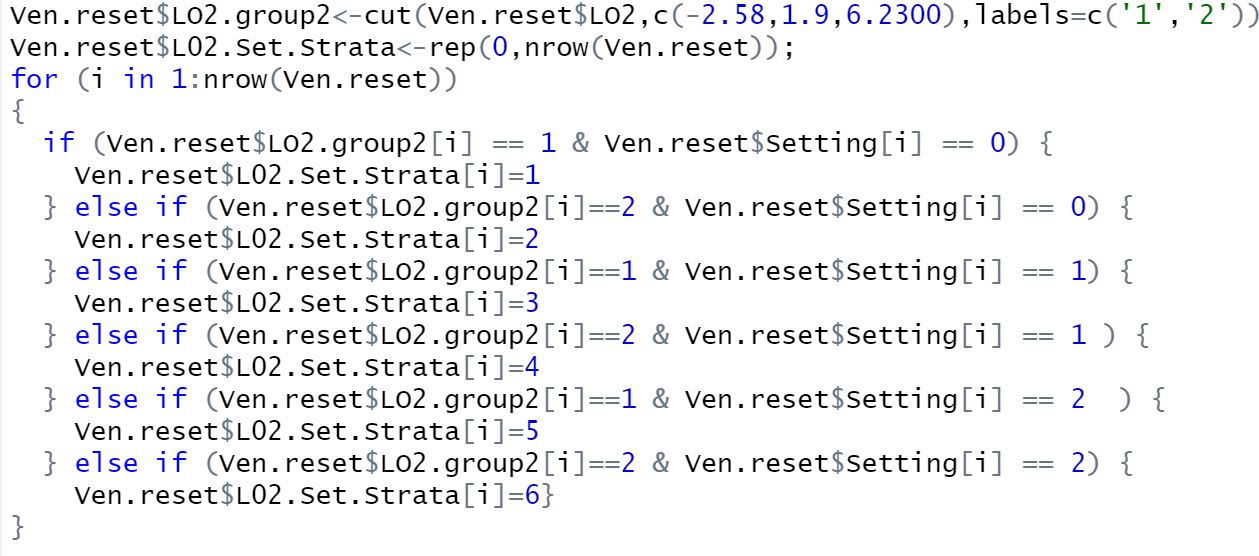
\includegraphics[scale=.5]{HW5code.JPG}
\end{center}
Use your stratification variable to test the appropriateness of the Weibull model with LO2 and Setting in the model. There are six curves each with only about 25 data points so the curves don't have to be ``perfect''.   
\end{enumerate} 
\item Fit a Weibull model with fixed shape parameter $p$ with LO2 and Setting in the model.  
\begin{enumerate}[i.] 
\item Are Setting and LO2 significant at $\alpha=0.05$? 
\item Give the Weibull AF model and  give a $95\%$ CI for the AF for Setting.   
\item Give the Weibull PH model and give a  $95\%$ CI for the HR for Setting
\end{enumerate}
\item Fit a Weibull model with fixed shape parameter $p$ with LO2 and Setting in the model and an interaction term between LO2 and Setting. 
\begin{enumerate}[i.]
\item Is interaction significant? Use the Wald test and likelihood ratio test. 
\item Give the AF model and HR for Setting at the first, second and third quartiles of LO2. 
\item Fit survival curves for Setting=0, 1 and 2 with LO2=mean(LO2) all on one plot. Use xlim=c(0,15) on your first plot. 
\item Based on your models and your plots, what can you say about the effect on survival of Setting adjusted for LO2?  
\end{enumerate} 
\item Fitting a log-logistic model to the Ventilator data set with just LO2. 
\begin{enumerate}[i.] 

\item Plot KM curves of LO2.group (with four strata as in previous homework) and conduct a log-rank test.
\item Use a log-log plot to show that a log-logistic model with fixed $p$  is not appropriate with just Setting in the model.
\item Use a log-log plot to show the appropriateness of the log-logistic model with fixed $p$ with just LO2.group in the model.
\item Fit an AFT log-logistic model with just LO2. Is LO2 a significant predictor? Give AF and $95\%$ CI for the AF.
\item Fit a PO log-logistic model with just LO2. Give the FOR and the $95\%$ CI for the FOR.
\item Plot estimated survival curves for LO2. Use the means of LO2.group for each of your curves. Compare your estimated survival curves to your KM curves. 
\end{enumerate} 
\end{enumerate} 



\end{document}

